% Intended LaTeX compiler: xelatex
\documentclass[10pt, svgnames]{beamer}
\usepackage{graphicx}
\usepackage{longtable}
\usepackage{wrapfig}
\usepackage{rotating}
\usepackage[normalem]{ulem}
\usepackage{amsmath}
\usepackage{amssymb}
\usepackage{capt-of}
\usepackage{hyperref}
\usetheme{focus}
\author{Sappinandana Akamphon}
\date{}
\title{Introduction to Theories of Failure}
\subtitle{ME 210: Mechanics of Materials}
\usepackage{booktabs}
\usepackage{pgfplots}
\pgfplotsset{compat=1.18}
\institute{Department of Mechanical Engineering, TSE}
\usetikzlibrary{patterns,shapes,arrows}
\setmathfont{Fira Math}
\AtBeginSection[]{\begin{frame}{Outline}\tableofcontents[currentsection]\end{frame}}
\hypersetup{
 pdfauthor={Sappinandana Akamphon},
 pdftitle={Introduction to Theories of Failure},
 pdfkeywords={},
 pdfsubject={},
 pdfcreator={Emacs 30.0.50 (Org mode 9.6)}, 
 pdflang={English}}
\begin{document}

\maketitle

\section{Material Failure}
\label{sec:orge334949}

\begin{frame}[label={sec:org5b130e9}]{Material Failure}
\begin{itemize}
\item Conditions in which materials lose its load-carrying capacity
\item 3 most prevalent failure modes
\begin{itemize}
\item Fracture \& Yield -- excessive stress causing molecular bond breakdown
\item Fatigue -- cumulative damage through repeated loadings
\item Buckling -- geometric instability from compressive load
\end{itemize}
\end{itemize}
\end{frame}

\section{Fracture \& Yield}
\label{sec:org8f6accb}

\begin{frame}[label={sec:org2d27338}]{Fracture \& Yield}
\begin{itemize}
\item Sufficiently high stress to overcome intermolecular bonds
\item Under uniaxial stress, a material fails when
\item Brittle material - broken molecular bond leads to material separation --  \emph{Fracture}
\item Ductile material - surface slip -- \emph{Yield}
\end{itemize}
\begin{center}
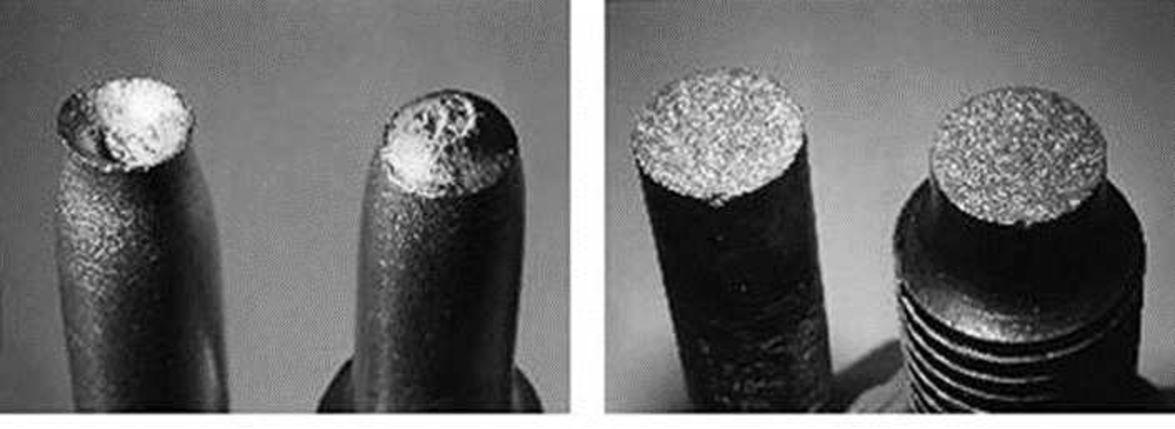
\includegraphics[width=.9\linewidth]{pictures/failure-ductile-brittle-sections.pdf}
\end{center}
\end{frame}

\begin{frame}[label={sec:org269d62a}]{Fracture}
\begin{itemize}
\item Material separation usually \emph{perpendicular} to the direction of stress -- predicted by normal stress
\item Where or what is the maximum normal stress in a given material? -- \(\sigma_1\) and \(\sigma_2\)
\end{itemize}

\begin{center}
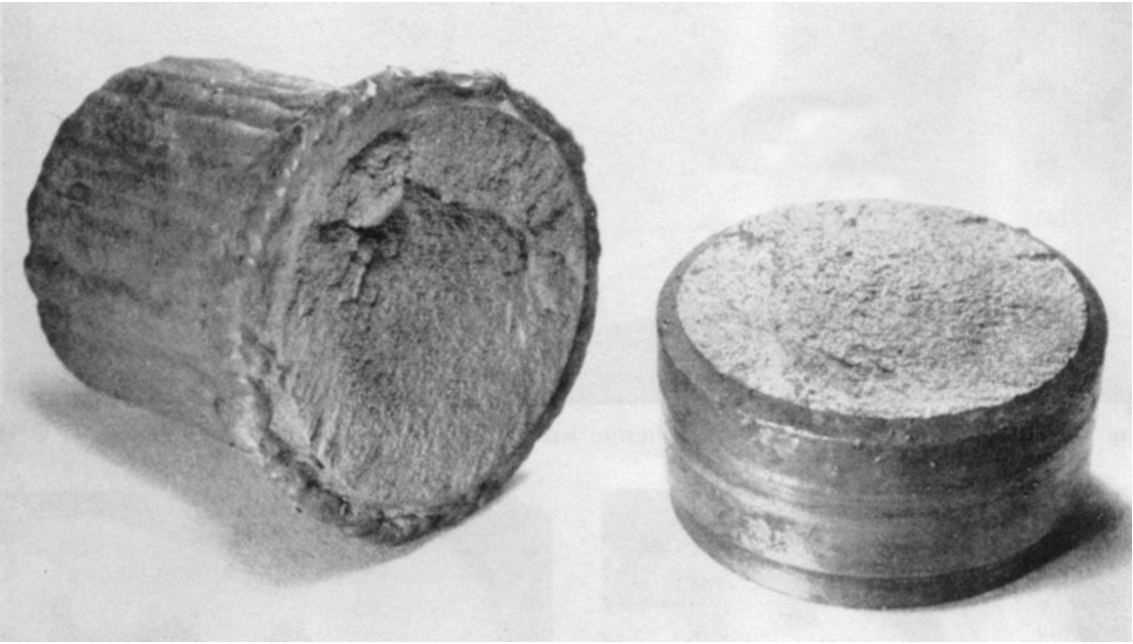
\includegraphics[width=.9\linewidth]{pictures/brittle-failure.pdf}
\end{center}
\end{frame}

\begin{frame}[label={sec:org373e478}]{Maximum Normal Stress Theory}
\begin{columns}
\begin{column}{0.4\columnwidth}
\begin{itemize}
\item In a nutshell: Determine if the maximum tensile and compressive stresses go beyond limit.
\item What is the limit?
\end{itemize}

For \(\sigma_1 > \sigma_2\)
$$\sigma_1 \leqslant S_{ut} $$
$$\sigma_2 \leqslant S_{uc} $$
\end{column}

\begin{column}{0.6\columnwidth}
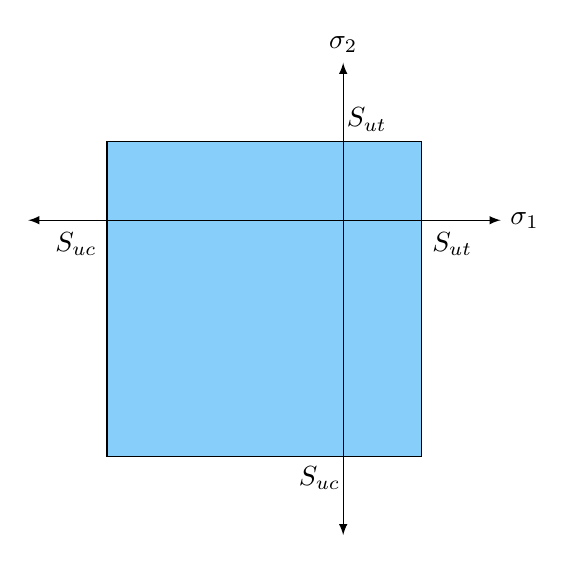
\begin{tikzpicture}[>=latex]
\node [draw, rectangle, xshift=-1cm, yshift=-1cm, fill=LightSkyBlue, minimum height=4cm, minimum width=4cm](sq){};
\draw [<->] (-4,0) --++ (0:6) node[right]{$\sigma_1$};
\node at (sq.east) [yshift=7mm, right] {$S_{ut}$};
\node at (sq.west) [yshift=7mm, left] {$S_{uc}$};
\node at (sq.north) [xshift=1.3cm, above] {$S_{ut}$};
\node at (sq.south) [xshift=7mm, below] {$S_{uc}$};
\draw [<->] (0,-4) --++ (90:6) node[above]{$\sigma_2$};
\end{tikzpicture}
\end{column}
\end{columns}
\end{frame}


\begin{frame}[label={sec:org2d9c084}]{Design Equation for MNST}
\begin{columns}
\begin{column}{0.4\columnwidth}
if \(\sigma_1 > \sigma_2\)
$$ \sigma_1 = \frac{S_{ut}}{N_s} $$
$$ \sigma_2 = \frac{S_{uc}}{N_s} $$
\end{column}

\begin{column}{0.6\columnwidth}
\begin{tikzpicture}[>=latex]
\node [draw, rectangle, xshift=-1cm, yshift=-1cm, minimum height=4cm, minimum width=4cm](sq){};
\node [draw, rectangle, xshift=-0.5cm, yshift=-0.5cm, minimum height=4cm, minimum width=4cm, scale=0.5, dashed]{};
\node [draw, rectangle, xshift=-.33cm, yshift=-.33cm, minimum height=4cm, minimum width=4cm, scale=0.33, dashed]{};
\draw [<->] (-4,0) --++ (0:6) node[right]{$\sigma_1$};
\node at (sq.east) [yshift=7mm, right] {$S_{ut}$};
\node at (sq.west) [yshift=7mm, left] {$S_{uc}$};
\node at (sq.north) [xshift=1.3cm, above] {$S_{ut}$};
\node at (sq.south) [xshift=7mm, below] {$S_{uc}$};
\draw [<->] (0,-4) --++ (90:6) node[above]{$\sigma_2$};
\end{tikzpicture}
\end{column}
\end{columns}
\end{frame}

\begin{frame}[label={sec:orgfdd40f0}]{Example: The Many Modes of Chalk Fracture}
\begin{itemize}
\item How do you think a blackboard chalk would break under axial load? bending? torsion?
\end{itemize}

\begin{center}
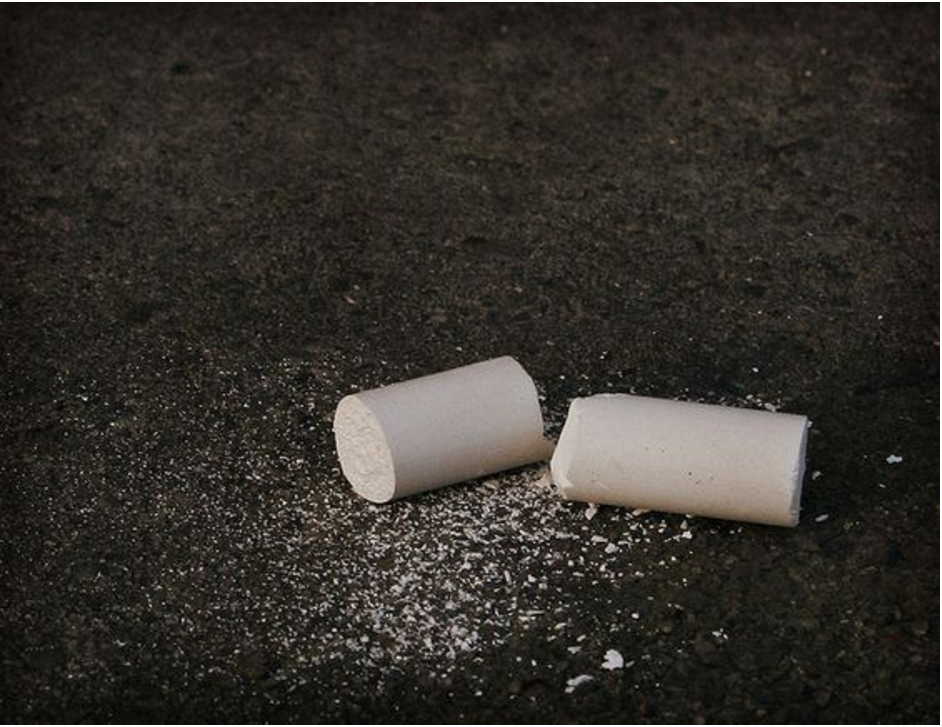
\includegraphics[width=.9\linewidth]{pictures/broken-chalk.pdf}
\end{center}
\end{frame}


\begin{frame}[label={sec:org7bfa2ad}]{Example: Brittle shaft under torsion}
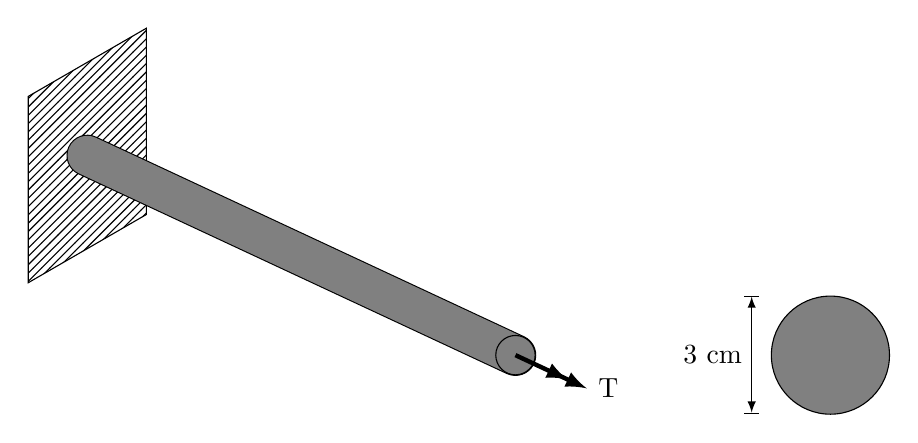
\begin{tikzpicture}[>=latex]
\node[draw, pattern=north east lines, trapezium, trapezium left angle=120, trapezium right angle=60, minimum height=1.5cm, rotate=90](wall){};
\draw [line cap=round, double=Grey, rounded corners=5mm, double distance=0.5cm] (wall.center) --++ (-25:6) node(end){};
\node at (end.center) [draw, ellipse, minimum height=0.5cm, minimum width=0.5cm](outerend){};
\draw [->>, ultra thick, >=latex] (end.center) --++ (-25:1) node[right]{T};
\node at (end.center) [xshift=4cm, circle, draw, minimum height=1.5cm, fill=Grey](outersect){};
\draw [|<->|, >=latex] (outersect.north) ++ (-180:1) --++ (-90:1.5) node[left, midway]{3 cm};
\end{tikzpicture}

\begin{itemize}
\item Determine maximum \(T\) when \(S_{ut}\) = 100 MPa and \(S_{uc}\) = 200 MPa
\end{itemize}
\end{frame}


\begin{frame}[label={sec:org589a043}]{Yield}
\begin{itemize}
\item Surface slip from material shearing -- predicted by shear stress
\item Two prevalent methods of determining yield
\item Maximum Shear Stress Theory (MSST or Tresca criteria)
\item Maximum Distortional Energy Theory (MDET or Von Mises criteria)
\end{itemize}
\end{frame}

\begin{frame}[label={sec:orgc59499a}]{Maximum Shear Stress Theory: Yield under Uniaxial Stress}
\begin{itemize}
\item The maximum shear stress in material cannot exceed max shear under uniaxial stress at yield -- what?
\item Under uniaxial stress, ductile material still fails due to shear stress, which can be derived as
\end{itemize}

$$\tau_{max} = \sqrt{\left(\frac{\sigma_x-\sigma_y}{2}\right)^2+\tau_{xy}^2}$$
$$\tau_{max} = \frac{S_y}{2}$$
\end{frame}


\begin{frame}[label={sec:org6b6ac4e}]{Maximum Shear Stress Theory: Small Shear?}
\begin{itemize}
\item What if material is in a state such that shear stress is small? Oh? Like how?
\item When \(|\sigma_x - \sigma_y|\) and \(\tau_{xy}\) are small
\item In that case, normal stresses cannot exceed \(S_y\)
\end{itemize}
$$\sigma_{1,2} < S_y $$
\end{frame}

\begin{frame}[label={sec:org4f43c00}]{Maximum Shear Stress Theory: In Summary}
\begin{columns}
\begin{column}{0.4\columnwidth}
\begin{itemize}
\item Combining the cases
\end{itemize}
$$\tau_{max} \leqslant \frac{S_y}{2}$$
$$\sigma_{1,2} \leqslant S_y $$
\end{column}

\begin{column}{0.6\columnwidth}
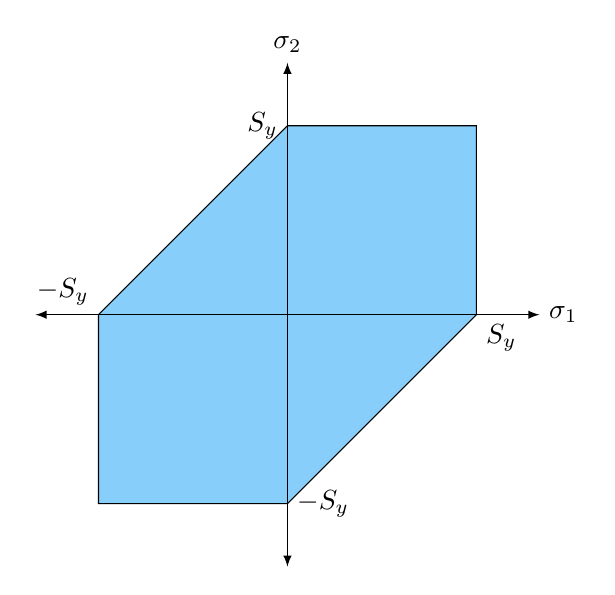
\begin{tikzpicture}[>=latex, scale=0.8]
\draw [fill=LightSkyBlue] (0,-3) node[right]{$-S_y$} -- (3,0) node[below right]{$S_y$} -- (3,3) -- (0,3) node[left]{$S_y$} -- (-3,0) node[above left]{$-S_y$} -- (-3,-3) -- cycle;
\draw [<->] (-4,0) --++ (0:8) node[right]{$\sigma_1$};
\draw [<->] (0,-4) --++ (90:8) node[above]{$\sigma_2$};
\end{tikzpicture}
\end{column}
\end{columns}
\end{frame}

\begin{frame}[label={sec:orgde2eec2}]{Design Equation for MSST}
\begin{gather*}
\tau_{max} = \frac{S_y}{2N_s}
\sigma_{1,2} = \frac{S_y}{N_s}
\end{gather*}

\begin{tikzpicture}[>=latex, scale=0.8]
\draw [dashed] (0,-3) node[right]{$-S_y$} -- (3,0) node[below right]{$S_y$} -- (3,3) -- (0,3) node[midway, below]{{$N_{s} = 1$}} node[left]{$S_y$} -- (-3,0) node[above left]{$-S_y$} -- (-3,-3) -- cycle;
\draw [dashed, scale=0.5] (0,-3) node[right]{} -- (3,0) node[below right]{} -- (3,3) -- (0,3) node[midway, below]{{2}} node[left]{} -- (-3,0) node[above left]{} -- (-3,-3) -- cycle;
\draw [dashed, scale=0.33] (0,-3) node[right]{} -- (3,0) node[below right]{} -- (3,3) -- (0,3) node[midway, below]{{3}} node[left]{} -- (-3,0) node[above left]{} -- (-3,-3) -- cycle;
\draw [<->] (-4,0) --++ (0:8) node[right]{$\sigma_1$};
\draw [<->] (0,-4) --++ (90:8) node[above]{$\sigma_2$};
\end{tikzpicture}
\end{frame}

\begin{frame}[label={sec:org51ef55f}]{Example: Ductile shaft under torsion}
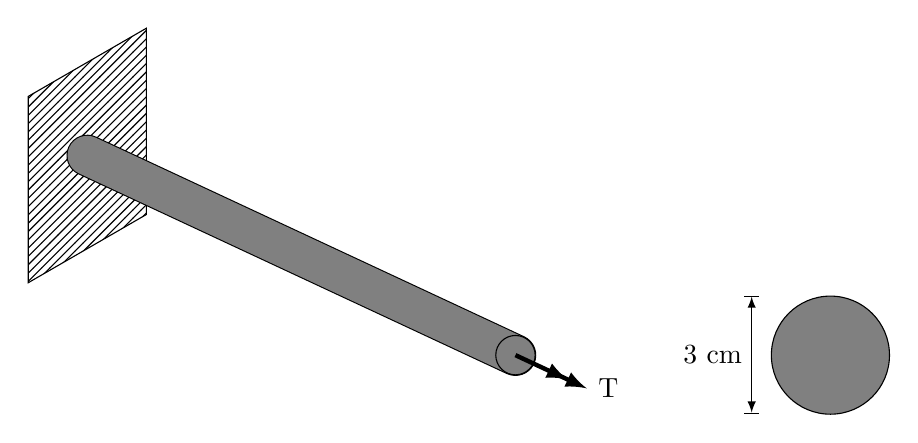
\begin{tikzpicture}[>=latex]
\node[draw, pattern=north east lines, trapezium, trapezium left angle=120, trapezium right angle=60, minimum height=1.5cm, rotate=90](wall){};
\draw [line cap=round, double=Grey, rounded corners=5mm, double distance=0.5cm] (wall.center) --++ (-25:6) node(end){};
\node at (end.center) [draw, ellipse, minimum height=0.5cm, minimum width=0.5cm](outerend){};
\draw [->>, ultra thick, >=latex] (end.center) --++ (-25:1) node[right]{T};
\node at (end.center) [xshift=4cm, circle, draw, minimum height=1.5cm, fill=Grey](outersect){};
\draw [|<->|, >=latex] (outersect.north) ++ (-180:1) --++ (-90:1.5) node[left, midway]{3 cm};
\end{tikzpicture}

\begin{itemize}
\item Determine maximum \(T\) when \(S_y\) = 100 MPa
\item Compare to brittle shaft problem
\end{itemize}
\end{frame}


\begin{frame}[label={sec:org04bcc3d}]{Distortional Energy Theory: Criteria}
\begin{itemize}
\item A deformed material has two types of strain energy
\item Dilatation strain energy \(\rightarrow\) change in volume
\item Distortion srain energy \(\rightarrow\) change in shape \(\rightarrow\) ductile failure
\item Criteria for failure: distortion strain energy equal to that during uniaxial stress yield
\end{itemize}
\end{frame}


\begin{frame}[label={sec:org4630475}]{Maximum Distortional Energy Theory: In Summary\}}
\begin{columns}
\begin{column}{0.4\columnwidth}
\begin{itemize}
\item Material will fail when
\end{itemize}
\begin{equation*}
\scalebox{1}{$\sigma_e = S_y$}
\end{equation*}
\begin{itemize}
\item where \(\sigma_e\) is the equivalent stress
\end{itemize}
\begin{align*}
\sigma_e &= \sqrt{\sigma_x^2 - \sigma_x\sigma_y + \sigma_y^2 + 3\tau_{xy}^2}
&= \sqrt{\sigma_1^2 - \sigma_1\sigma_2 + \sigma_2^2}
\end{align*}
\end{column}

\begin{column}{0.6\columnwidth}
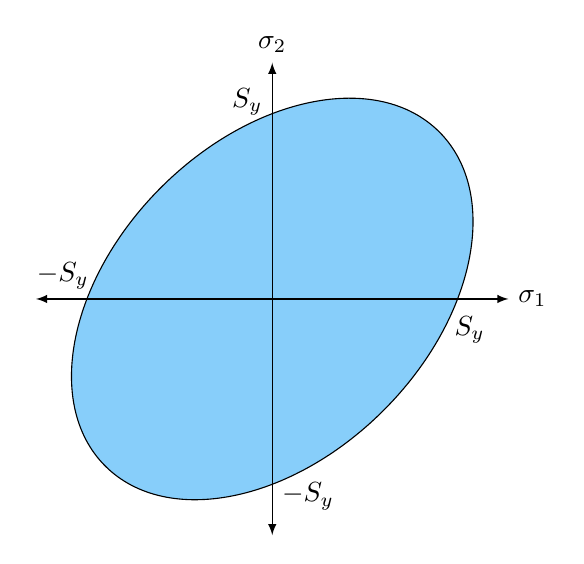
\begin{tikzpicture}[>=latex]
\node [draw, ellipse, fill=LightSkyBlue, minimum width=6cm, minimum height=4cm, rotate=45](el){};
\node at (el.north east)[left, xshift=-5mm]{$S_y$};
\node at (el.south east)[below, yshift=-6mm]{$S_y$};
\node at (el.north west)[above left, yshift=5mm, xshift=3mm]{$-S_y$};
\node at (el.south west)[right, xshift=5mm]{$-S_y$};
\draw [<->] (-3,0) --++ (0:6) node[right]{$\sigma_1$};
\draw [<->] (0,-3) --++ (90:6) node[above]{$\sigma_2$};
\end{tikzpicture}
\end{column}
\end{columns}
\end{frame}


\begin{frame}[label={sec:org17af14b}]{Design Equation for MDET\}}
\begin{columns}
\begin{column}{0.4\columnwidth}
$$ \sigma_e = \frac{S_y}{N_s} $$
\end{column}

\begin{column}{0.6\columnwidth}
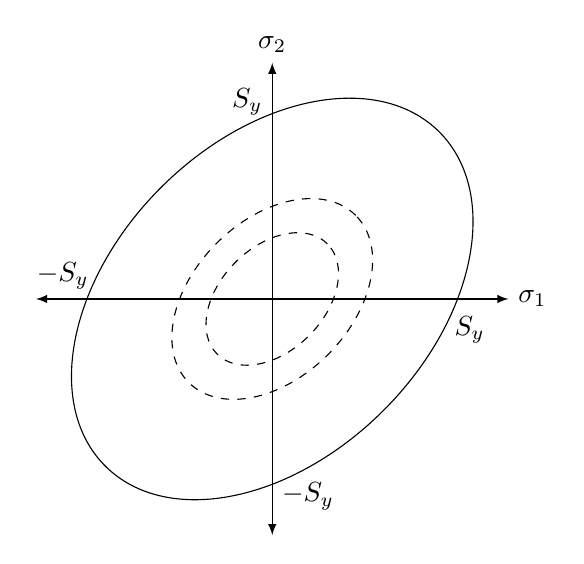
\begin{tikzpicture}[>=latex]
\node [draw, ellipse, minimum width=6cm, minimum height=4cm, rotate=45](el){};
\node [draw, ellipse, minimum width=6cm, minimum height=4cm, rotate=45, scale=0.5, dashed]{};
\node [draw, ellipse, minimum width=6cm, minimum height=4cm, rotate=45, scale=0.33, dashed]{};
\node at (el.north east)[left, xshift=-5mm]{$S_y$};
\node at (el.south east)[below, yshift=-6mm]{$S_y$};
\node at (el.north west)[above left, yshift=5mm, xshift=3mm]{$-S_y$};
\node at (el.south west)[right, xshift=5mm]{$-S_y$};
\draw [<->] (-3,0) --++ (0:6) node[right]{$\sigma_1$};
\draw [<->] (0,-3) --++ (90:6) node[above]{$\sigma_2$};
\end{tikzpicture}
\end{column}
\end{columns}
\end{frame}


\begin{frame}[label={sec:org0e5d43f}]{Comparison Between Different Criteria}
\scriptsize
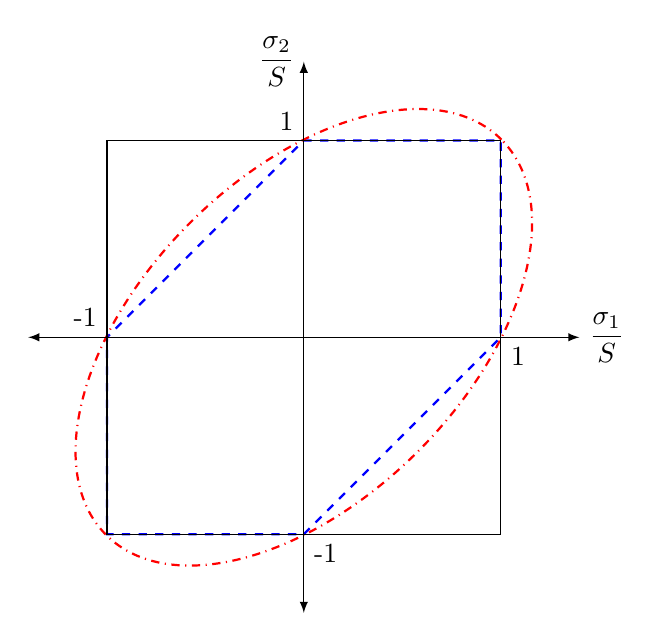
\begin{tikzpicture}[>=latex]
\draw [dashed, thick, Blue] (0,-2.5) node[below right, Black]{-1} -- (2.5,0) node[below right, Black]{1} -- (2.5,2.5) -- (0,2.5) node[above left, Black]{1} -- (-2.5,0) node[above left, Black]{-1} -- (-2.5,-2.5) -- cycle;
\node [draw, dash dot, thick, Red, ellipse, minimum height=4.1cm, minimum width=7.1cm, rotate=45]{};
\node [draw, rectangle, minimum height=5cm, minimum width=5cm]{};
\draw [<->] (-3.5,0) --++ (0:7) node[right]{$\dfrac{\sigma_1}{S}$};
\draw [<->] (0,-3.5) --++ (90:7) node[left]{$\dfrac{\sigma_2}{S}$};
\end{tikzpicture}
\end{frame}

\section{Fatigue}
\label{sec:org8985086}

\begin{frame}[label={sec:orgddddc38}]{Fatigue}
\begin{columns}
\begin{column}{0.5\columnwidth}
\begin{center}
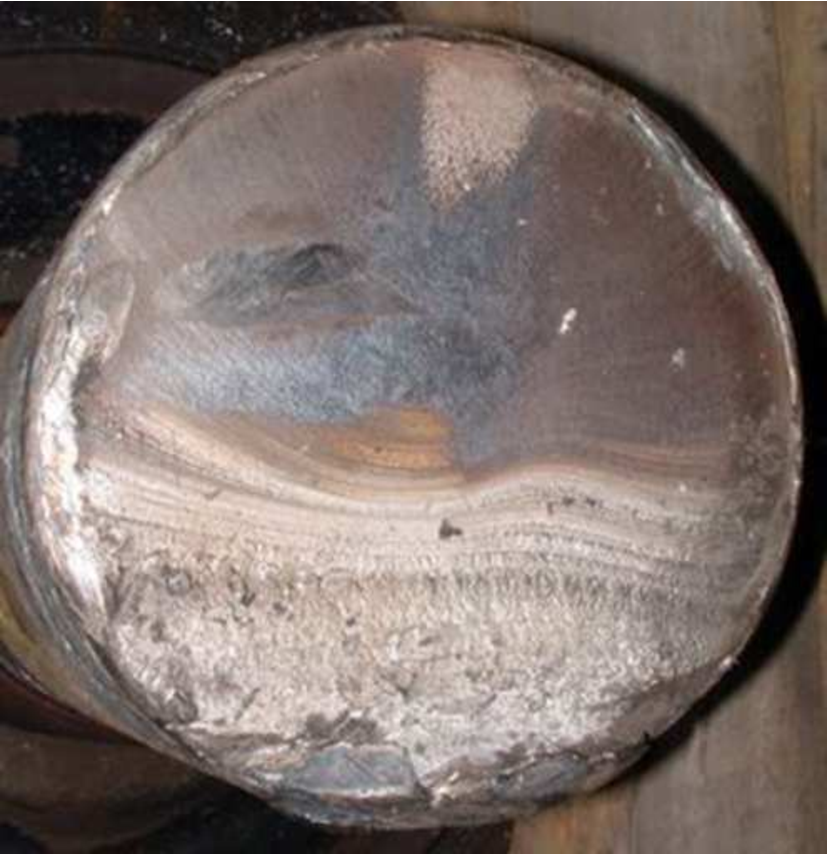
\includegraphics[width=.9\linewidth]{pictures/fatigue-failure.pdf}
\end{center}
\end{column}

\begin{column}{0.5\columnwidth}
\begin{itemize}
\item Failure of material based on repeated or fluctuating loads
\item Smaller than ultimate tensile stress
\item Crack starts small and grows increasingly fast as load is repeated
\end{itemize}
\end{column}
\end{columns}
\end{frame}

\begin{frame}[label={sec:org4aaf2cc}]{Repeated Loading}
\begin{itemize}
\item Much like a periodic function, there are mainly two important features of a repeated loading concerning fatigue

\item Stress amplitude \(\sigma_a = \dfrac{\sigma_{\max} - \sigma_{\min}}{2}\)
\item Mean (average) stress \(\sigma_m = \dfrac{\sigma_{\max} + \sigma_{\min}}{2}\)
\end{itemize}

\begin{center}
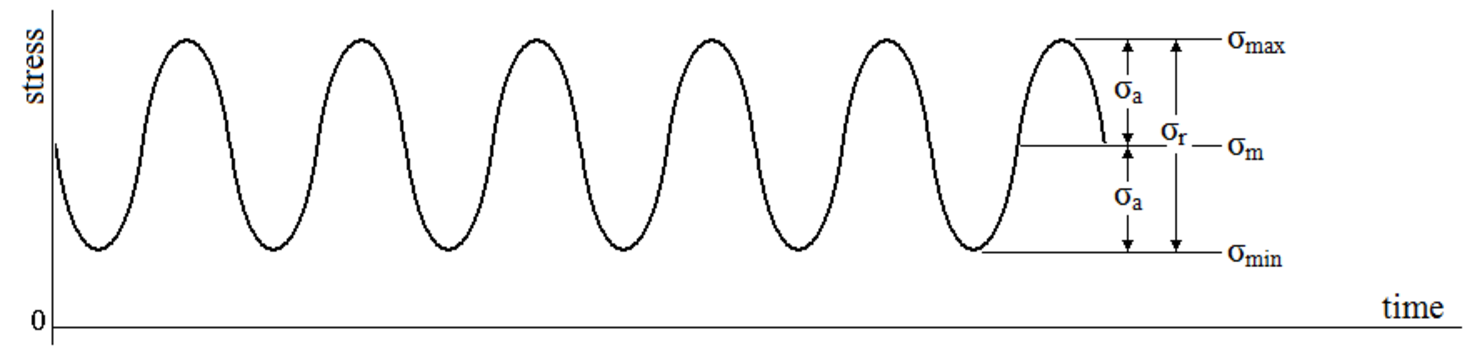
\includegraphics[width=.9\linewidth]{pictures/fluctuating-load.pdf}
\end{center}
\end{frame}

\begin{frame}[label={sec:orgf449462}]{Testing for Fatigue\}}
\begin{columns}
\begin{column}{0.5\columnwidth}
\begin{center}
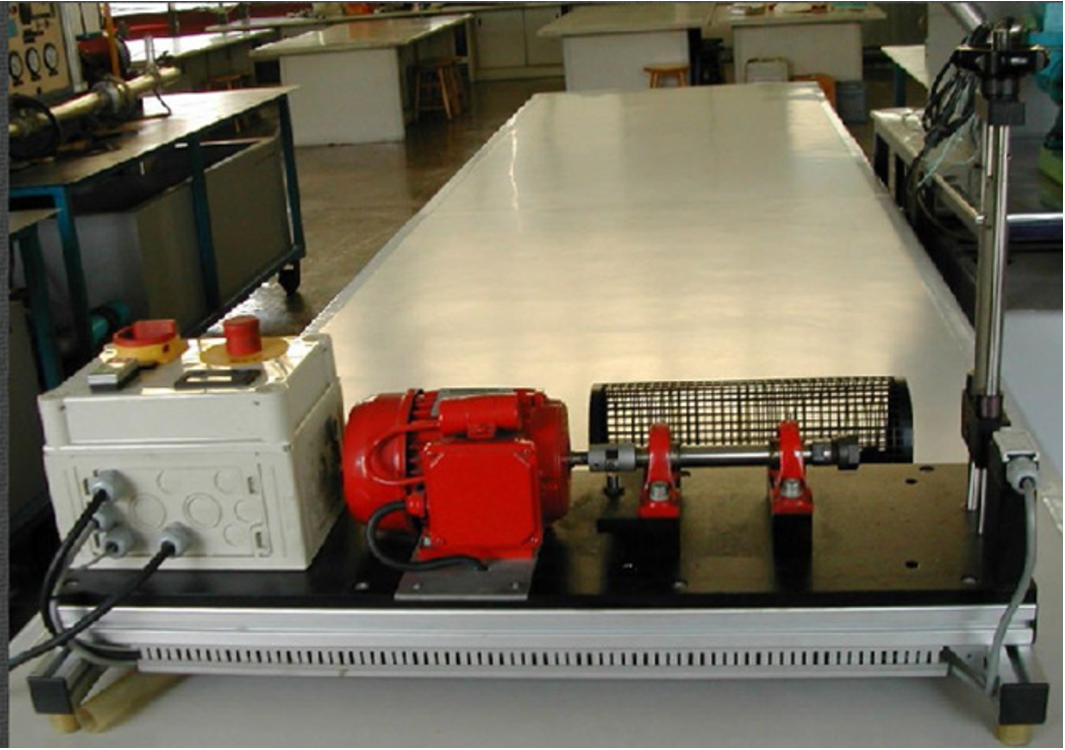
\includegraphics[width=.9\linewidth]{pictures/rotating-beam-exp.pdf}
\end{center}
\end{column}

\begin{column}{0.5\columnwidth}
\begin{center}
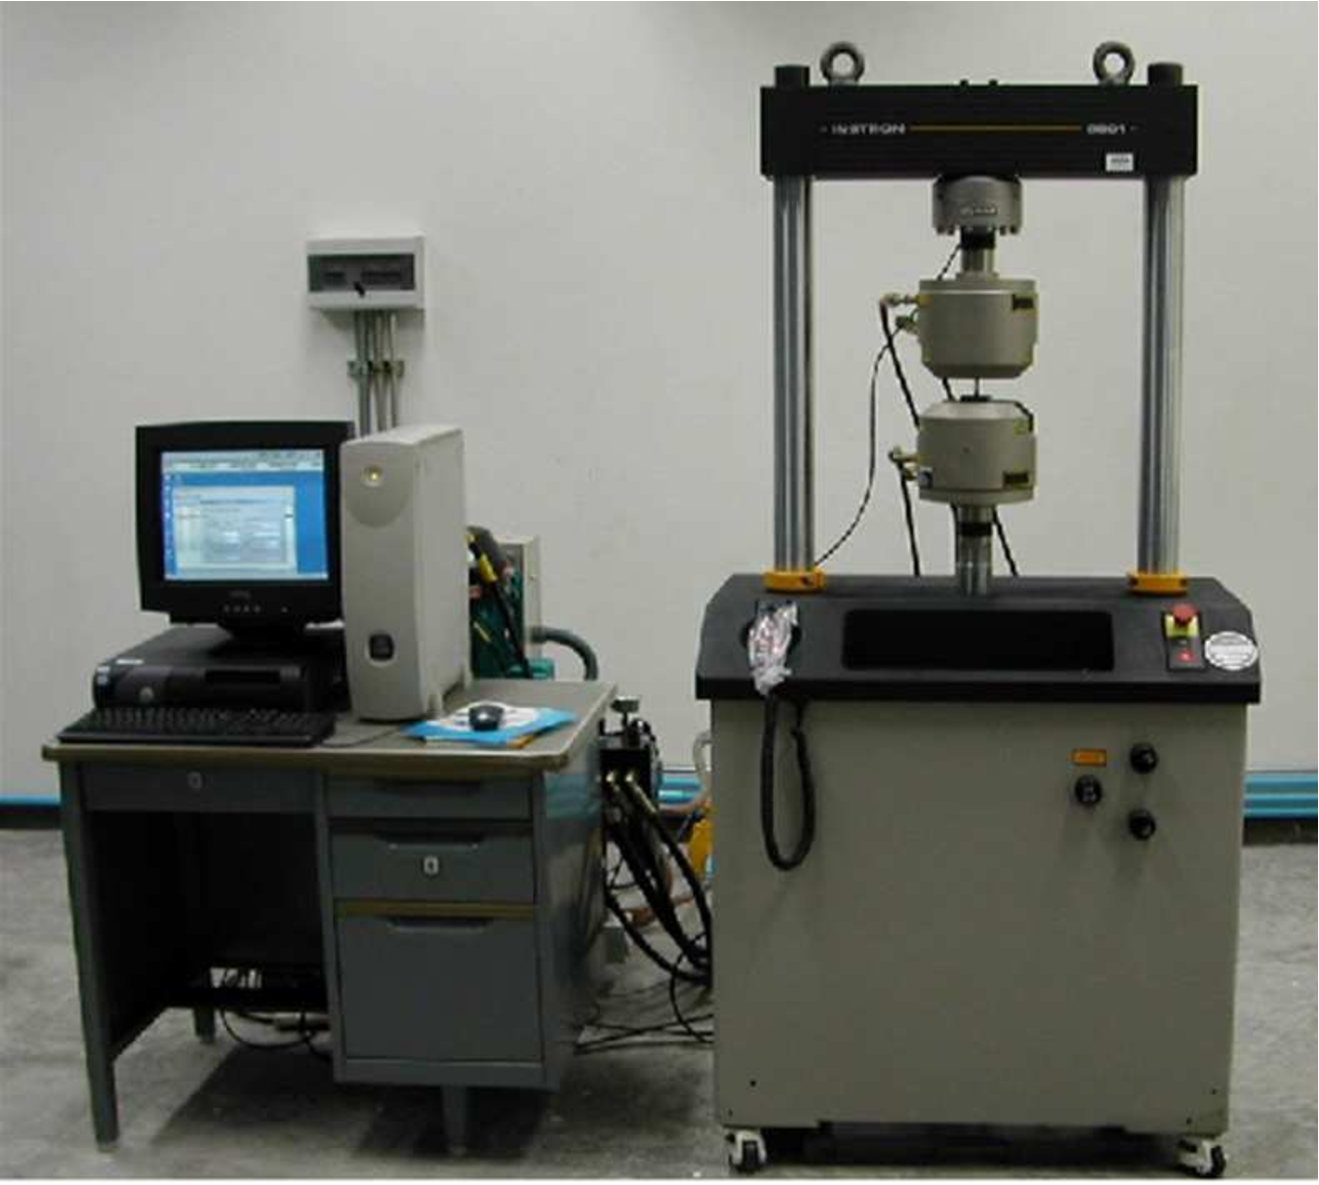
\includegraphics[width=.9\linewidth]{pictures/univ-tensile-test.pdf}
\end{center}
\end{column}
\end{columns}
\end{frame}

\begin{frame}[label={sec:orgc00b598}]{S-N or Endurance Diagram}
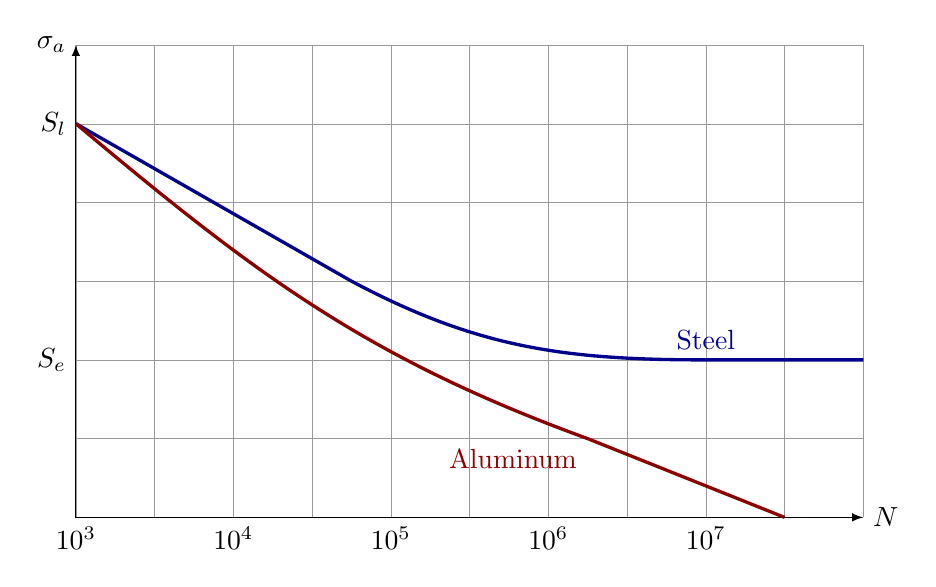
\begin{tikzpicture}[>=latex]
\draw[ultra thin,color=Black!40] (0,0) grid (10,6);
\draw[<->]  (0,6) node [left] {$\sigma_a$} -- (0,5) node[left]{$S_l$} -- (0,2) node[left]{$S_e$} -- (0,0) node[below] {$10^3$} -- (2,0)  node[below]{$10^4$} -- (4,0) node[below]{$10^5$} -- (6,0) node[below]{$10^6$} -- (8,0) node[below]{$10^7$} -- (10,0) node[right] {$N$};
\draw[very thick, DarkBlue] (0,5) to (3.5,3) to [out=-28,in=-180] (8,2) node[above]{Steel} to (10,2);
\draw[very thick, DarkRed] (0,5) to [out=-40,in=160] (6.5,1) node[below left]{Aluminum} to (9,0);
\end{tikzpicture}
\end{frame}


\begin{frame}[label={sec:org56f4b7f}]{Endurance Limit or Fatigue Limit}
Endurance limit is the maximum stress amplitude for which the part will last \(10^7\) cycles

For steel
\begin{align*}
	Bending: S_e &\approx 0.5S_{ut} \\
	Axial: S_e &\approx 0.45S_{ut} \\
	Torsion: S_e &\approx 0.29S_{ut}
\end{align*}

Aluminum does \emph{not} have endurance limit (is that a good thing?)
\end{frame}


\begin{frame}[label={sec:org2f76b9c}]{Low cycle fatigue \((N < 1000)\)\}}
\begin{itemize}
\item Steel parts will last for \(\approx\) 1000 cycles if the applied stress amplitude is
\end{itemize}

\begin{columns}
\begin{column}{0.5\columnwidth}
\begin{align*}
Bending: S_l &\approx 0.9S_{ut}
Axial: S_l &\approx 0.75S_{ut}
Torsion: S_l &\approx 0.72S_{ut}
\end{align*}
\end{column}

\begin{column}{0.5\columnwidth}
\begin{center}
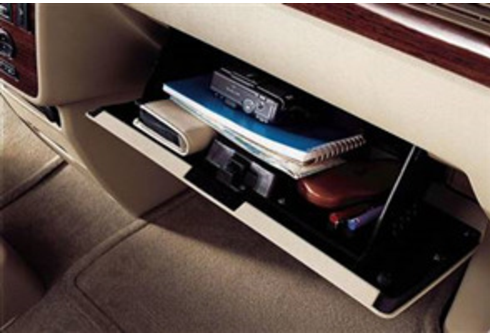
\includegraphics[width=.9\linewidth]{pictures/glove-comp.pdf}
\end{center}
\begin{center}
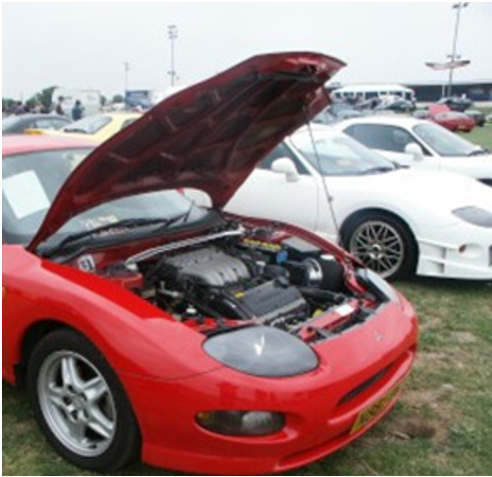
\includegraphics[width=.9\linewidth]{pictures/car-hood.pdf}
\end{center}
\end{column}
\end{columns}
\end{frame}

\begin{frame}[label={sec:orga941175}]{High cycle fatigue \((10^3 < N < 10^6)\)}
\begin{itemize}
\item Steel parts will last for about \(N\) cycles if fatigue stress \(\sigma_a\)
\end{itemize}

\begin{align*}
	\sigma_a &= 10^c N^b \\
	b &= -\dfrac{1}{3}   \log\dfrac{S_l}{S_e} \\
	c &= \log \dfrac{S_l^2}{S_e}
\end{align*}
\end{frame}


\begin{frame}[label={sec:org40f48c5}]{Example: bar under cyclic axial load}
A bar is made of steel with \(S_{ut}\) = 300 MPa and is cyclically loaded axially between -200 and 200 MPa. Determine the useful life of this bar.
\end{frame}



\begin{frame}[label={sec:org177beed}]{Modified Endurance Limit}
\begin{itemize}
\item Experiments find that endurance limits of materials vary due to their conditions
\end{itemize}

\begin{align*}
S'_e &= K_f K_s K_t S_e  [10pt]
K_f &= \text{finishing factor}
K_s &= \text{size factor}
K_t &= \text{thermal factor}
\end{align*}
\end{frame}


\begin{frame}[label={sec:org7c2db6f}]{Fatigue Failure with Nonzero Average Stress}
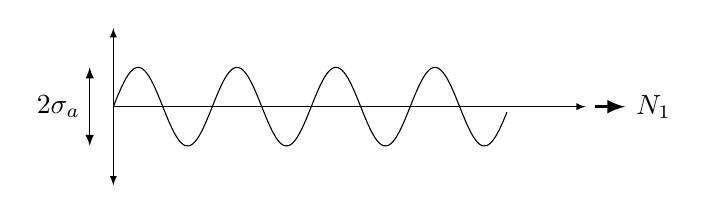
\begin{tikzpicture}[>=latex]
\draw [domain=0:5, scale=1, smooth, samples=100] plot ({\x}, {0.5*sin (5*\x r)});
\draw [->, very thin] (0,0) --++ (0:6) node(A){};
\draw [<->, very thin] (0,-1) --++ (90:2);
\draw [<->] (-0.3, -0.5) --++ (90:1) node[midway, left]{$2\sigma_a$};
\draw [->, very thick] (A) --++ (0:0.5) node[right]{$N_1$};
\end{tikzpicture}

\begin{tikzpicture}[>=latex]
\draw [domain=0:5, scale=1, smooth, samples=100] plot ({\x}, {0.5*sin (5*\x r) + 0.4});
\draw [->, very thin] (0,0) --++ (0:6);
\draw [<->, very thin] (0,-1) --++ (90:2);
\draw [<->] (-0.45, -0.1) --++ (90:1) node[midway, left]{$2\sigma_a$};
\draw [->, very thick] (A) --++ (0:0.5) node[right]{$N_2$};
\end{tikzpicture}

\begin{itemize}
\item \(N_1 > N_2 ?\)
\item By how much?
\end{itemize}
\end{frame}


\begin{frame}[label={sec:orgb34f063}]{Average Stress Correction Equations}
\begin{itemize}
\item Soderberg relation
\end{itemize}
$$ \dfrac{\sigma_a}{S_e} + \dfrac{\sigma_m}{S_y} = \dfrac{1}{N_s} $$
\begin{itemize}
\item Gerber relation
\end{itemize}
$$ \dfrac{\sigma_a}{S_e} + \left( \dfrac{\sigma_m}{S_{ut}} \right)^2 = \dfrac{1}{N_s} $$
\begin{itemize}
\item Goodman relation
\end{itemize}
$$ \dfrac{\sigma_a}{S_e} + \dfrac{\sigma_m}{S_{ut}} = \dfrac{1}{N_s} $$

These are called \emph{constant life lines}.
\end{frame}


\begin{frame}[label={sec:org65b9f8b}]{Average Stress Correction Comparison}
\begin{center}
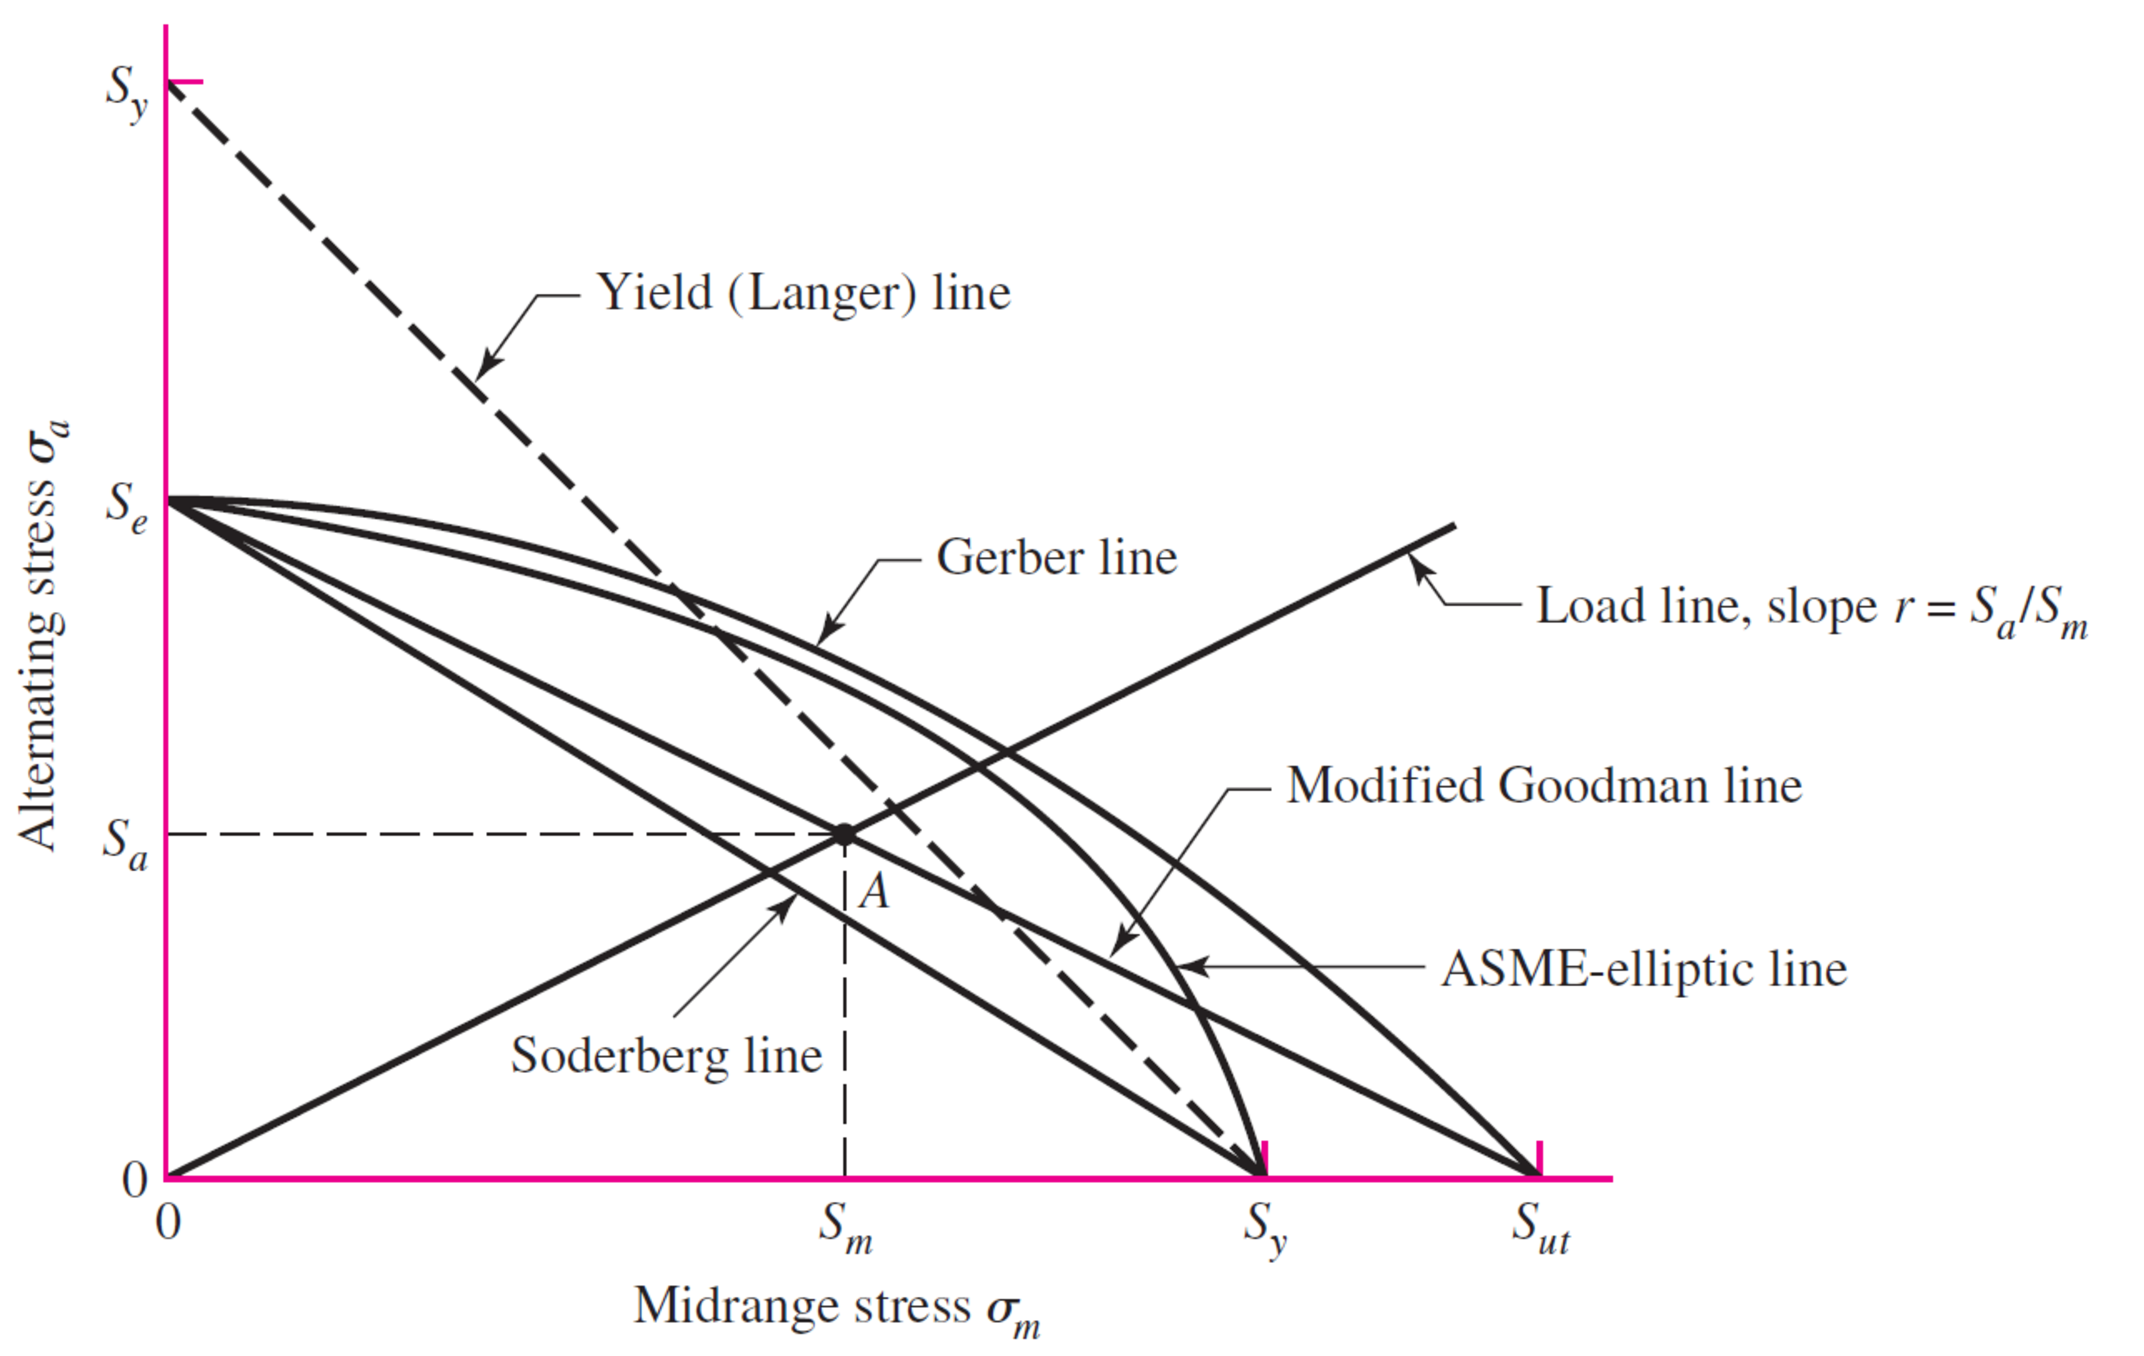
\includegraphics[width=.9\linewidth]{pictures/stresscorrection.pdf}
\end{center}
\end{frame}


\begin{frame}[label={sec:org2e392df}]{Example: Bar under nonzero average stress}
A cylindrical rod under a periodic tensile load between 0 and 8000 N. Material of the rod has \(S_y\) = 427 MPa  \(S_{ut}\) = 748 MPa. Determine the suitable diameter of the rod. Use Soderberg relation.

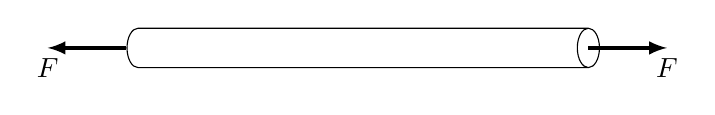
\begin{tikzpicture}[>=latex]
\node[draw, cylinder, minimum height=6cm, minimum width=5mm, inner sep=4](beam){};
\draw [->, very thick] (beam.east) ++ (180:0.15) --++ (0:1) node[below]{$F$};
\draw [->, very thick] (beam.west) --++ (180:1) node[below]{$F$};
\end{tikzpicture}
\end{frame}

\section{Buckling}
\label{sec:org5a47ea1}

\begin{frame}[label={sec:orgf3b8c39}]{What is Buckling?}
\begin{itemize}
\item Failure due to instability of column under compressive load
\item Restoring moment \(<\) moment from compressive load
\end{itemize}

\begin{center}
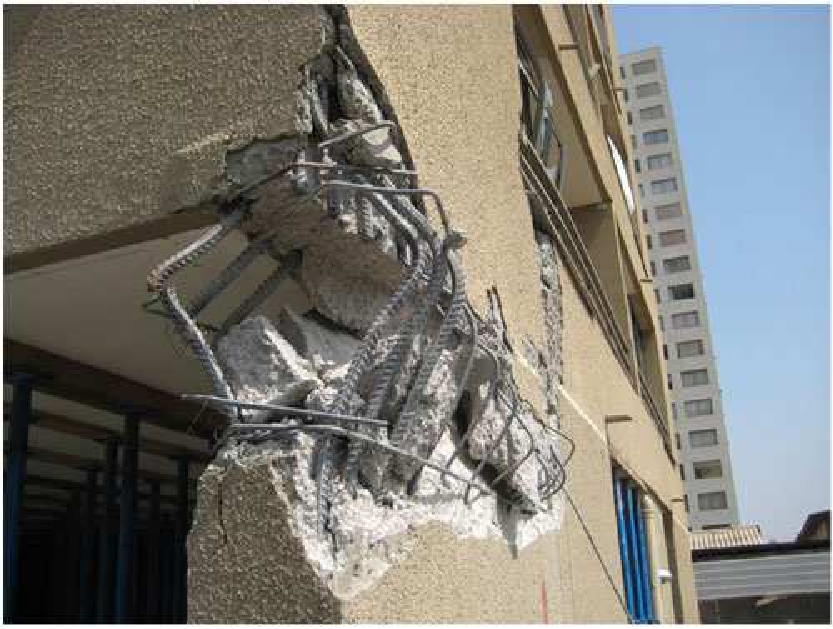
\includegraphics[width=.9\linewidth]{pictures/buckled-column.pdf}
\end{center}
\end{frame}

\begin{frame}[label={sec:org7b0684a}]{Governing Equation of Buckling}
\begin{columns}
\begin{column}{0.5\columnwidth}
\begin{center}
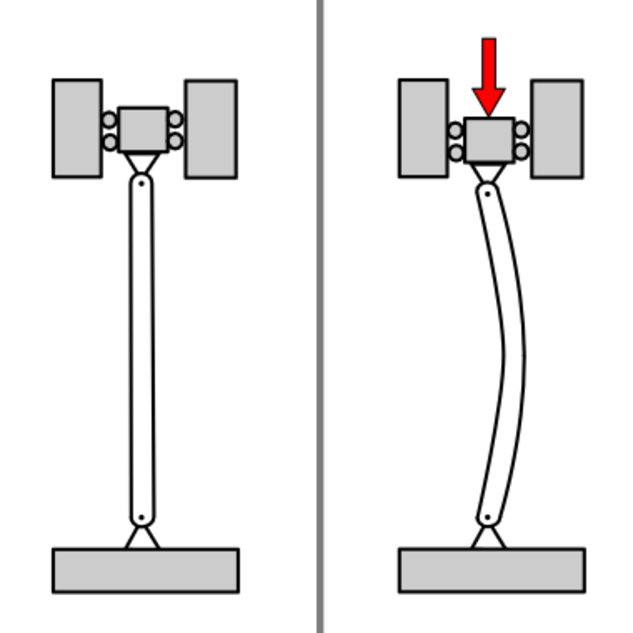
\includegraphics[width=.9\linewidth]{pictures/buckling-governing-eq.pdf}
\end{center}
\end{column}

\begin{column}{0.5\columnwidth}
\begin{gather*}
M(x) = -Pv \\
EI\dfrac{d^2 v}{d x^2} = -Pv \\
\dfrac{d^2 v}{d x^2} + \left( \dfrac{P}{EI} \right) v = 0
\end{gather*}
\end{column}
\end{columns}
\end{frame}

\begin{frame}[label={sec:orga1e2fe8}]{Solving for Buckling}
The generalized solution takes the form

$$ \scalebox{1}{$ v(x) = A \cos \sqrt{\dfrac{P}{EI}}   x + B \sin \sqrt{\dfrac{P}{EI}}    x $} $$

Solving for \(A\) and \(B\), we know that \(v(0) = 0\) and \(v(L) = 0\)

$$ v(0) = 0 = A \cos 0 + B \sin 0 $$
$$ A = 0 $$
\end{frame}

\begin{frame}[label={sec:org4d9a58c}]{Boring Solution}
$$ v(L) = 0 $$
$$ B \sin  \sqrt{\frac{P}{EI}}   L = 0 $$

$$ B = 0 $$
$$ v(x) = 0 \rightarrow trivial   solution $$
The solution is correct, but not helpful in determining the load \(P\)

So what's the interesting solution then?
\end{frame}

\begin{frame}[label={sec:orge7e0d72}]{Interesting Solution}
Ok, so \(B\) can't be 0, which means

$$  \sin  \sqrt{\frac{P}{EI}}   L = 0  $$
$$  \sqrt{\frac{P}{EI}}   L = n\pi $$

$$ P = \dfrac{n^2 \pi^2 E I}{L^2}, n = 1, 2, \dots $$
Now this is so much more helpful and interesting.
\end{frame}

\begin{frame}[label={sec:org26bef01}]{Critical Load and Corresponding Mode Shape}
For \(n = 1\)
$$ P_{crit} = \dfrac{\pi^2 E I}{L^2} $$
This is called \emph{Euler load} or \emph{Critical load}.

What does the corresponding buckled column look like?
$$ v(x) = B \sin \sqrt{\frac{P}{EI}}   x = B \sin \dfrac{n \pi x}{L} $$
\end{frame}

\begin{frame}[label={sec:org75158ae}]{Mode Shapes for Buckled Columns}
\begin{center}
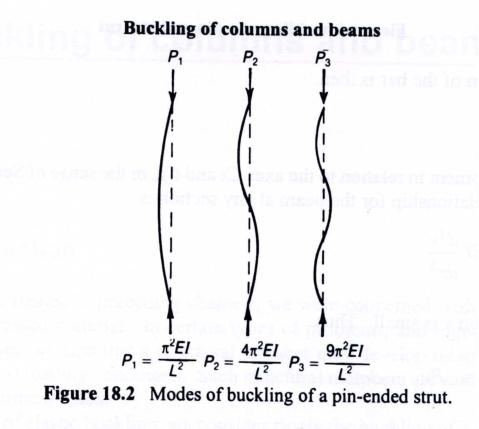
\includegraphics[width=.9\linewidth]{pictures/buckling-mode.pdf}
\end{center}
\end{frame}

\begin{frame}[label={sec:org4c5cd51}]{Buckling in Fixed - Free Supports}
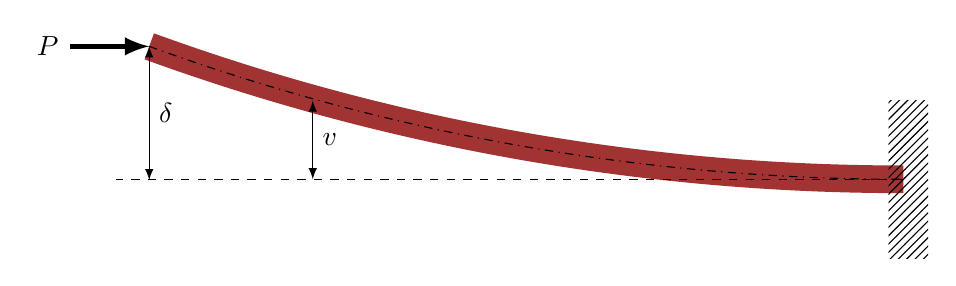
\begin{tikzpicture}[>=latex]
\draw [DarkRed!80, line width=10pt] (-4,0) node(A){} arc (-110:-90:28) node[inner sep=0pt](B){};
\draw [dash dot] (-4,0) arc (-110:-90:28);
\node at (B.west) [anchor=west,rectangle, pattern=north east lines, minimum height=2cm, minimum width=0.5cm]{};
\draw [<-, line width=2pt] (A.center) -- ++ (180:1) node[left]{$P$};
\draw [dashed] (B.center) -- ++ (180:10);
\draw [<->] (A.center)  --++ (-90:1.7) node[midway, right]{$\delta$};
\draw [<->] (B.center)  ++ (-7.5,0) --++ (90:1) node[midway, right]{$v$};
\end{tikzpicture}

\begin{gather*}
M = P(\delta - v)  \\[5pt]
EI\frac{d^2v}{dx^2} = P(\delta  - v)  \\[5pt]
\frac{d^2v}{dx^2} + \frac{P}{EI}v = \frac{P}{EI}\delta
\end{gather*}
\end{frame}

\begin{frame}[label={sec:org3991441}]{Governing Differential Equation Solution}
This equation is nonhomogeneous \(\rightarrow\) the solution consists of both a complementary and particular solutions.

\[v = C_1\sin \left( \sqrt \frac{P}{EI} x \right) + C_2\cos \left( \sqrt \frac{P}{EI} x \right) + \delta \]

Solving for constants of integration using \(v(x = 0) = 0\) and \(v(x = L) = \delta\), we have that

\[\delta \cos \left( \sqrt \frac{P}{EI} L \right) = 0\]
\end{frame}


\begin{frame}[label={sec:org28d7511}]{}
The nontrivial solution indicates that

\begin{gather*}
\cos \left( \sqrt \frac{P}{EI} L \right) = 0 \\
\sqrt \frac{P}{EI} L = \frac{(2n + 1)\pi}{2}
\end{gather*}

The smallest critical load (\(n = 0\)) is

$$ P_{cr} = \frac{\pi ^2EI}{4L^2} $$
\end{frame}

\begin{frame}[label={sec:orgf09e3a8}]{Generalized Critical Load}
\begin{align*}
P_{cr} &= \frac{\pi^2 EI}{L_e^2} \\
L_e &= KL \\
\end{align*}
\begin{align*}
L_e &= \text{effective length} \\
K &= \text{constant depending on supports} \\
\end{align*}
\end{frame}

\begin{frame}[label={sec:org3a81eff}]{Buckling in Other Types of Supports}
\begin{center}
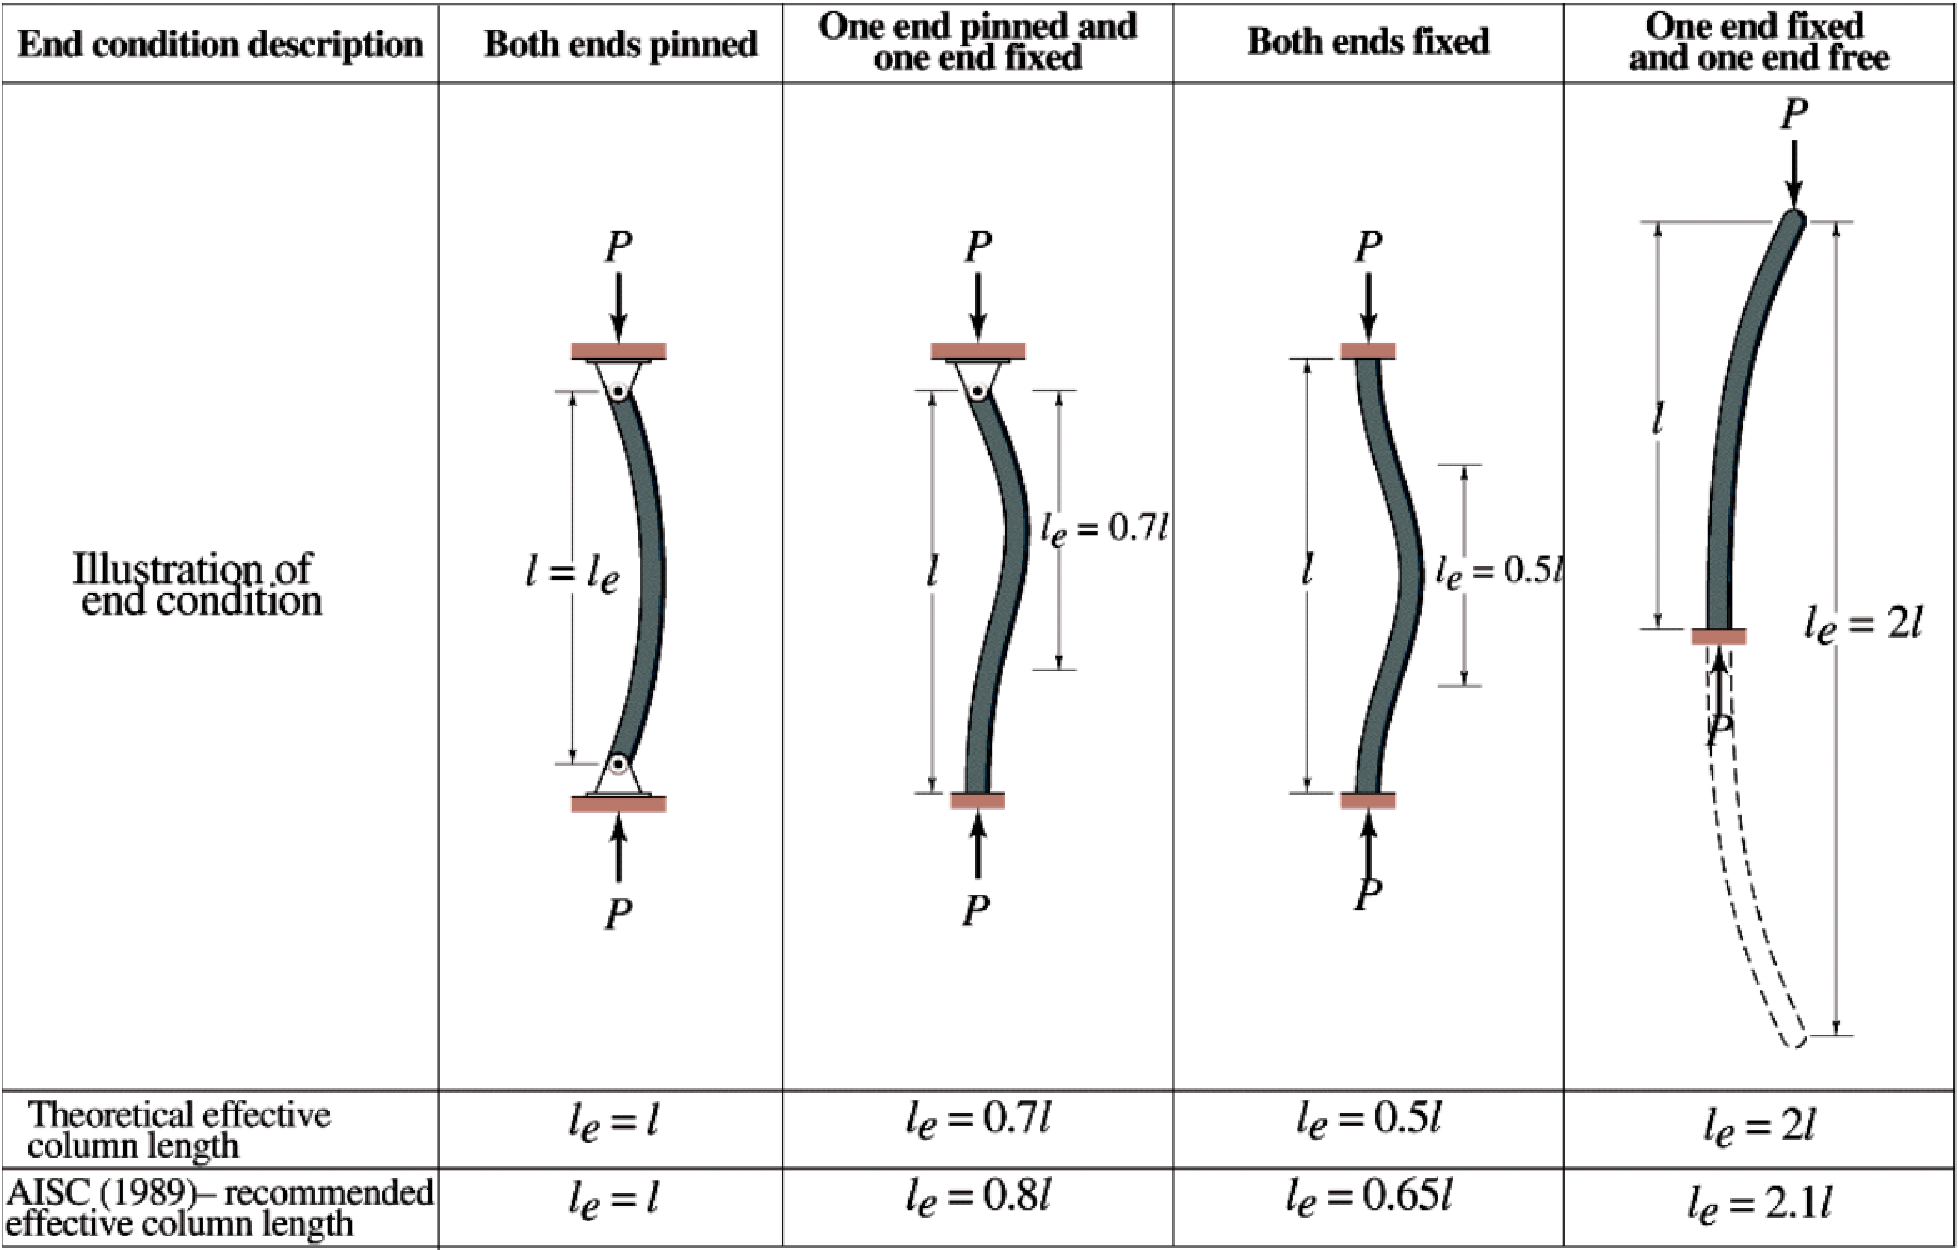
\includegraphics[width=.9\linewidth]{pictures/buckling-other-supports.pdf}
\end{center}
\end{frame}


\begin{frame}[label={sec:org8c47220}]{Slenderness Ratio \(\lambda\)}
\begin{itemize}
\item How \emph{slender} is a column?
\end{itemize}

$$ \lambda = \frac{KL}{r_g} $$
where \(r_g\) = radius of gyration = \(\sqrt{\dfrac{I}{A}}\)

\begin{align*}
\sigma_{cr} &= \frac{P_{cr}}{A} \\
&= \frac{\pi^2 EI}{AL_e^2} \\
&= \frac{\pi^2 E}{\lambda^2}
\end{align*}
\end{frame}


\begin{frame}[label={sec:orgdf6cb40}]{Buckling Design Equation}
\begin{align*}
P_{allow} = \frac{P_{cr}}{N_{s}} &= \frac{\pi^2 EI}{N_{s}L_e^2} \\
\sigma_{allow} = \frac{\sigma_{cr}}{N_{s}} &= \frac{\pi^2 E}{ N_{s}\lambda^2}
\end{align*}
\end{frame}

\begin{frame}[label={sec:org795164a}]{Example: Buckling of a Railroad Track in the Sun}
\begin{columns}
\begin{column}{0.6\columnwidth}
\begin{center}
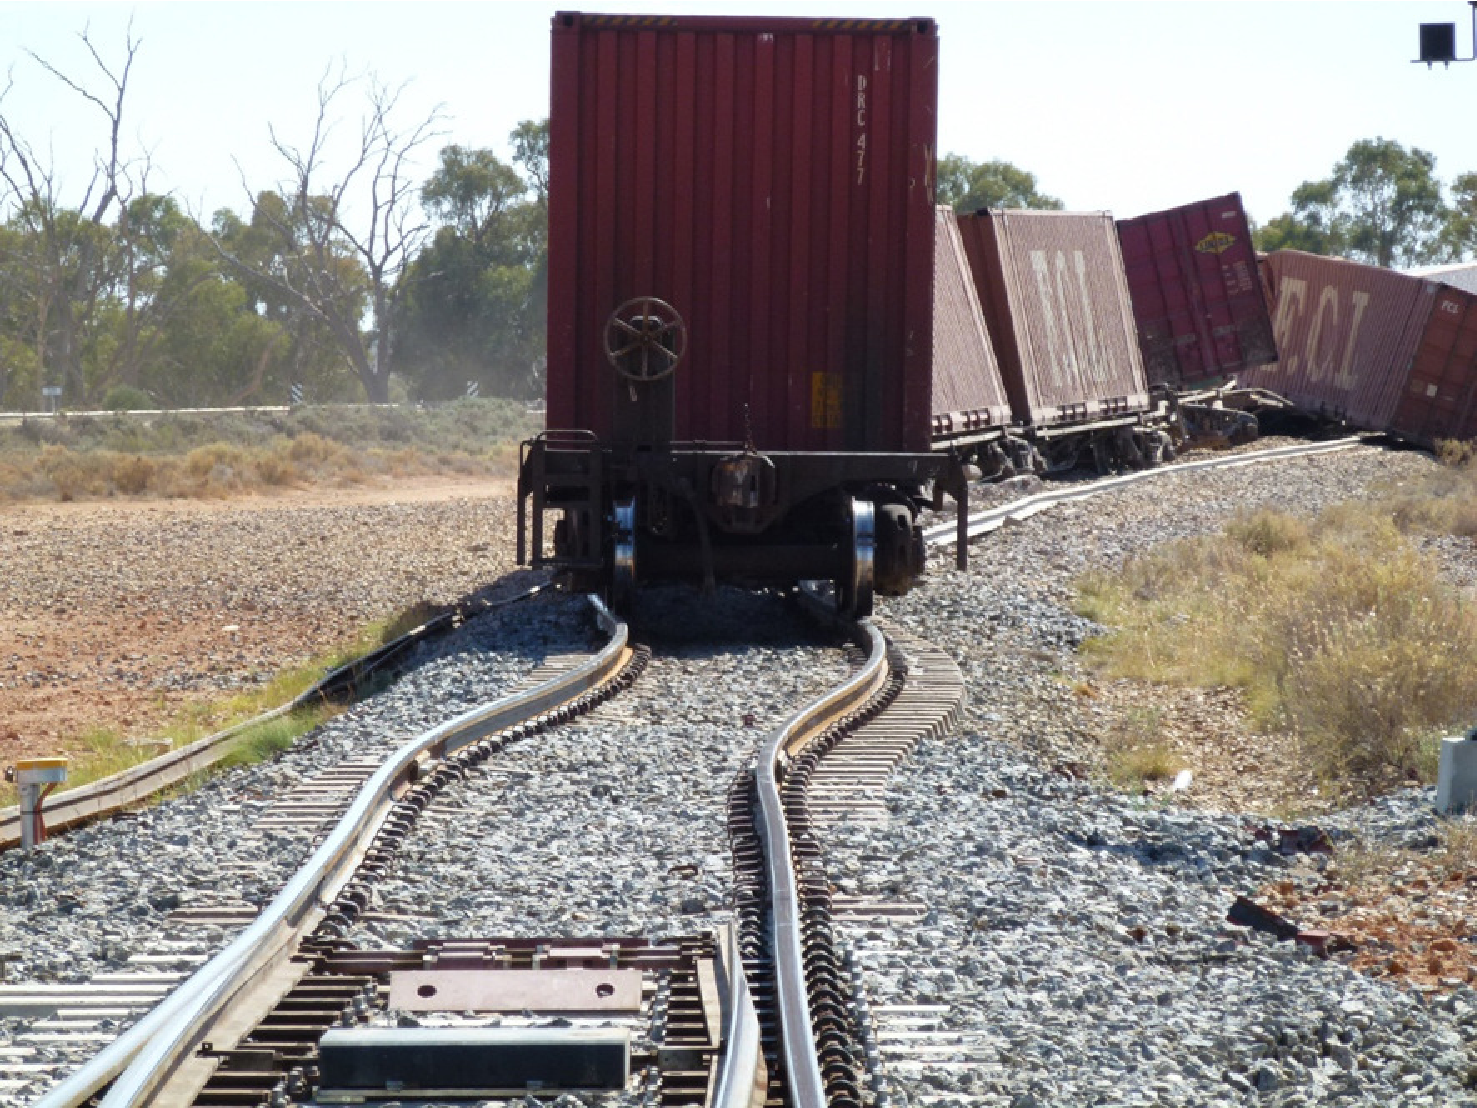
\includegraphics[width=.9\linewidth]{pictures/buckled-railroad.pdf}
\end{center}
\end{column}

\begin{column}{0.4\columnwidth}
\begin{itemize}
\item What parameters do we need to determine required \(\Delta T\) to cause buckling?
\item \(E, A, I, L?\)
\item \(\alpha?\)
\end{itemize}
\end{column}
\end{columns}
\end{frame}
\end{document}